%-------------------------
% Author: Rifat Arefin
%------------------------
\documentclass[letterpaper,11pt]{article}
\usepackage{ragged2e} %used to justify the text
\usepackage{latexsym}
\usepackage{xcolor}
\usepackage[empty]{fullpage}
\usepackage{titlesec}
\usepackage{marvosym}
\usepackage[hidelinks]{hyperref}
\usepackage{fancyhdr}
\usepackage[english]{babel}
\usepackage{tabularx}
\usepackage{fontawesome5}
\usepackage{multicol}
\usepackage{enumitem}
\usepackage{graphicx}
\graphicspath{{../img/}{assets/img/}}

\setlength{\multicolsep}{-3.0pt}
\setlength{\columnsep}{-1pt}
\input{glyphtounicode}

%----------FONT OPTIONS----------
% serif
\usepackage{CormorantGaramond}
\usepackage{charter}

\pagestyle{fancy}
\fancyhf{} % clear all header and footer fields
\fancyfoot{}
\renewcommand{\headrulewidth}{0pt}
\renewcommand{\footrulewidth}{0pt}

% Adjust margins
\addtolength{\oddsidemargin}{-0.5in}
\addtolength{\evensidemargin}{-0.5in}
\addtolength{\textwidth}{1.0in}
\addtolength{\topmargin}{-0.5in} % Top margin
\addtolength{\textheight}{1.0in}
\setlength{\footskip}{6pt}

\urlstyle{same}

\raggedbottom
\raggedright
\setlength{\tabcolsep}{0in}

% Define custom colors
\definecolor{NavyBlue}{RGB}{0, 51, 102}
\definecolor{DarkGreen}{RGB}{0, 100, 0}
\definecolor{DarkRed}{RGB}{139, 0, 0}
\definecolor{Teal}{RGB}{0, 128, 128}
\definecolor{SlateGray}{RGB}{112, 128, 144}
\definecolor{urlcolor}{RGB}{0, 45, 179}

% This lines are used to customize the hyper links
\hypersetup{
    colorlinks=true,
    linkcolor=red,
    urlcolor= NavyBlue
}

% Sections formatting
\titleformat{\section}{
  \vspace{-5pt}\scshape\raggedright\large\bfseries
}{}{0em}{}[\color{black}\titlerule \vspace{-5pt}]

% Ensure that generate pdf is machine readable/ATS parsable
\pdfgentounicode=1

%-------------------------
% Custom commands
%-------------------------

\newcommand{\resumeSubSubheading}[2]{
    \item
    \begin{tabular*}{1.0\textwidth}{l@{\extracolsep{\fill}}r}
        \textit{\small#1} & \textit{\small #2} \\
    \end{tabular*}\vspace{-7pt}
}

\newcommand{\resumeSubheading}[4]{
  \item
    \begin{tabular*}{1.0\textwidth}[t]{l@{\extracolsep{\fill}}r}
        \textbf{#1} & \textbf{\small #2} \\
        \textit{\small#3} & \textit{\small #4} \\
    \end{tabular*}
}

\newcommand{\researchProjectItem}[3]{
    \item
        \noindent
        \begin{minipage}[t]{0.8\textwidth}
            #1 \vspace{3pt}
        \end{minipage}%
        \hfill%
        \begin{minipage}[t]{0.2\textwidth}
            \raggedleft
            \raisebox{0pt}[0pt][0pt]{\textbf{\small #2}}
        \end{minipage}
        \begin{minipage}[t]{1.0\textwidth}
            \small #3
        \end{minipage}
        \vspace{-5pt}
}

\newcommand{\resumeSubItem}[1]{\resumeItem{#1}\vspace{-4pt}}
\renewcommand\labelitemi{$\vcenter{\hbox{\tiny$\bullet$}}$}
\renewcommand\labelitemii{$\vcenter{\hbox{\tiny$\bullet$}}$}

\newcommand{\resumeSubHeadingListStart}{\begin{itemize}[leftmargin=0.0in, label={}]}
\newcommand{\resumeSubHeadingListEnd}{\end{itemize}}

\newcommand{\resumeItemListStart}{\begin{itemize}[leftmargin=0.15in]}
\newcommand{\resumeItemListEnd}{\end{itemize}}

\newcommand{\ExperienceItemListStart}{\begin{itemize}[leftmargin=0.3in]}
\newcommand{\ExperienceItemListEnd}{\end{itemize}}

\newcommand{\resumeItem}[1]{\item {#1}}
\newcommand{\resumeItemSmall}[1]{\item \small{#1}}

%-------------------------------------------
%%%%%%%%%%%%%%%%%%%%  RESUME Starts Here  %%%%%%%%%%%%%%%%%%%%
\begin{document}

%%%%%%%%%%%%%%%%%%%%  Title  %%%%%%%%%%%%%%%%%%%%
\noindent
\begin{tabularx}{\textwidth}{@{}lX@{}}
    \begin{minipage}[t]{0.8\textwidth}
        \vspace{5pt}
        \begin{flushleft}
            {\Huge \scshape Rifat Arefin} \\
            \vspace{5pt}
            Road-1, House-2, Block-F, Mirpur-2, Dhaka-1216 \\
            \vspace{5pt}
            \raisebox{-0.0\height}\faPhone\ +880--1881445919 ~ \\
            \vspace{5pt}
            \href{mailto:arefinrifat786@gmail.com}{\raisebox{-0.1\height}\faEnvelope\  \underline{arefinrifat786@gmail.com}} ~ \\
            \vspace{7pt}
            \href{https://www.linkedin.com/in/rifatarefin32/}{\raisebox{-0.1\height}\faLinkedin\ \underline{linkedin.com/in/Rifat Arefin}}  ~
            \href{https://github.com/RifatArefin32}{\raisebox{-0.1\height}\faGithub\ \underline{github.com/RifatArefin32}}
        \end{flushleft}
    \end{minipage}
    &
    \begin{minipage}[t]{0.2\textwidth}
        \vspace{-30pt}
        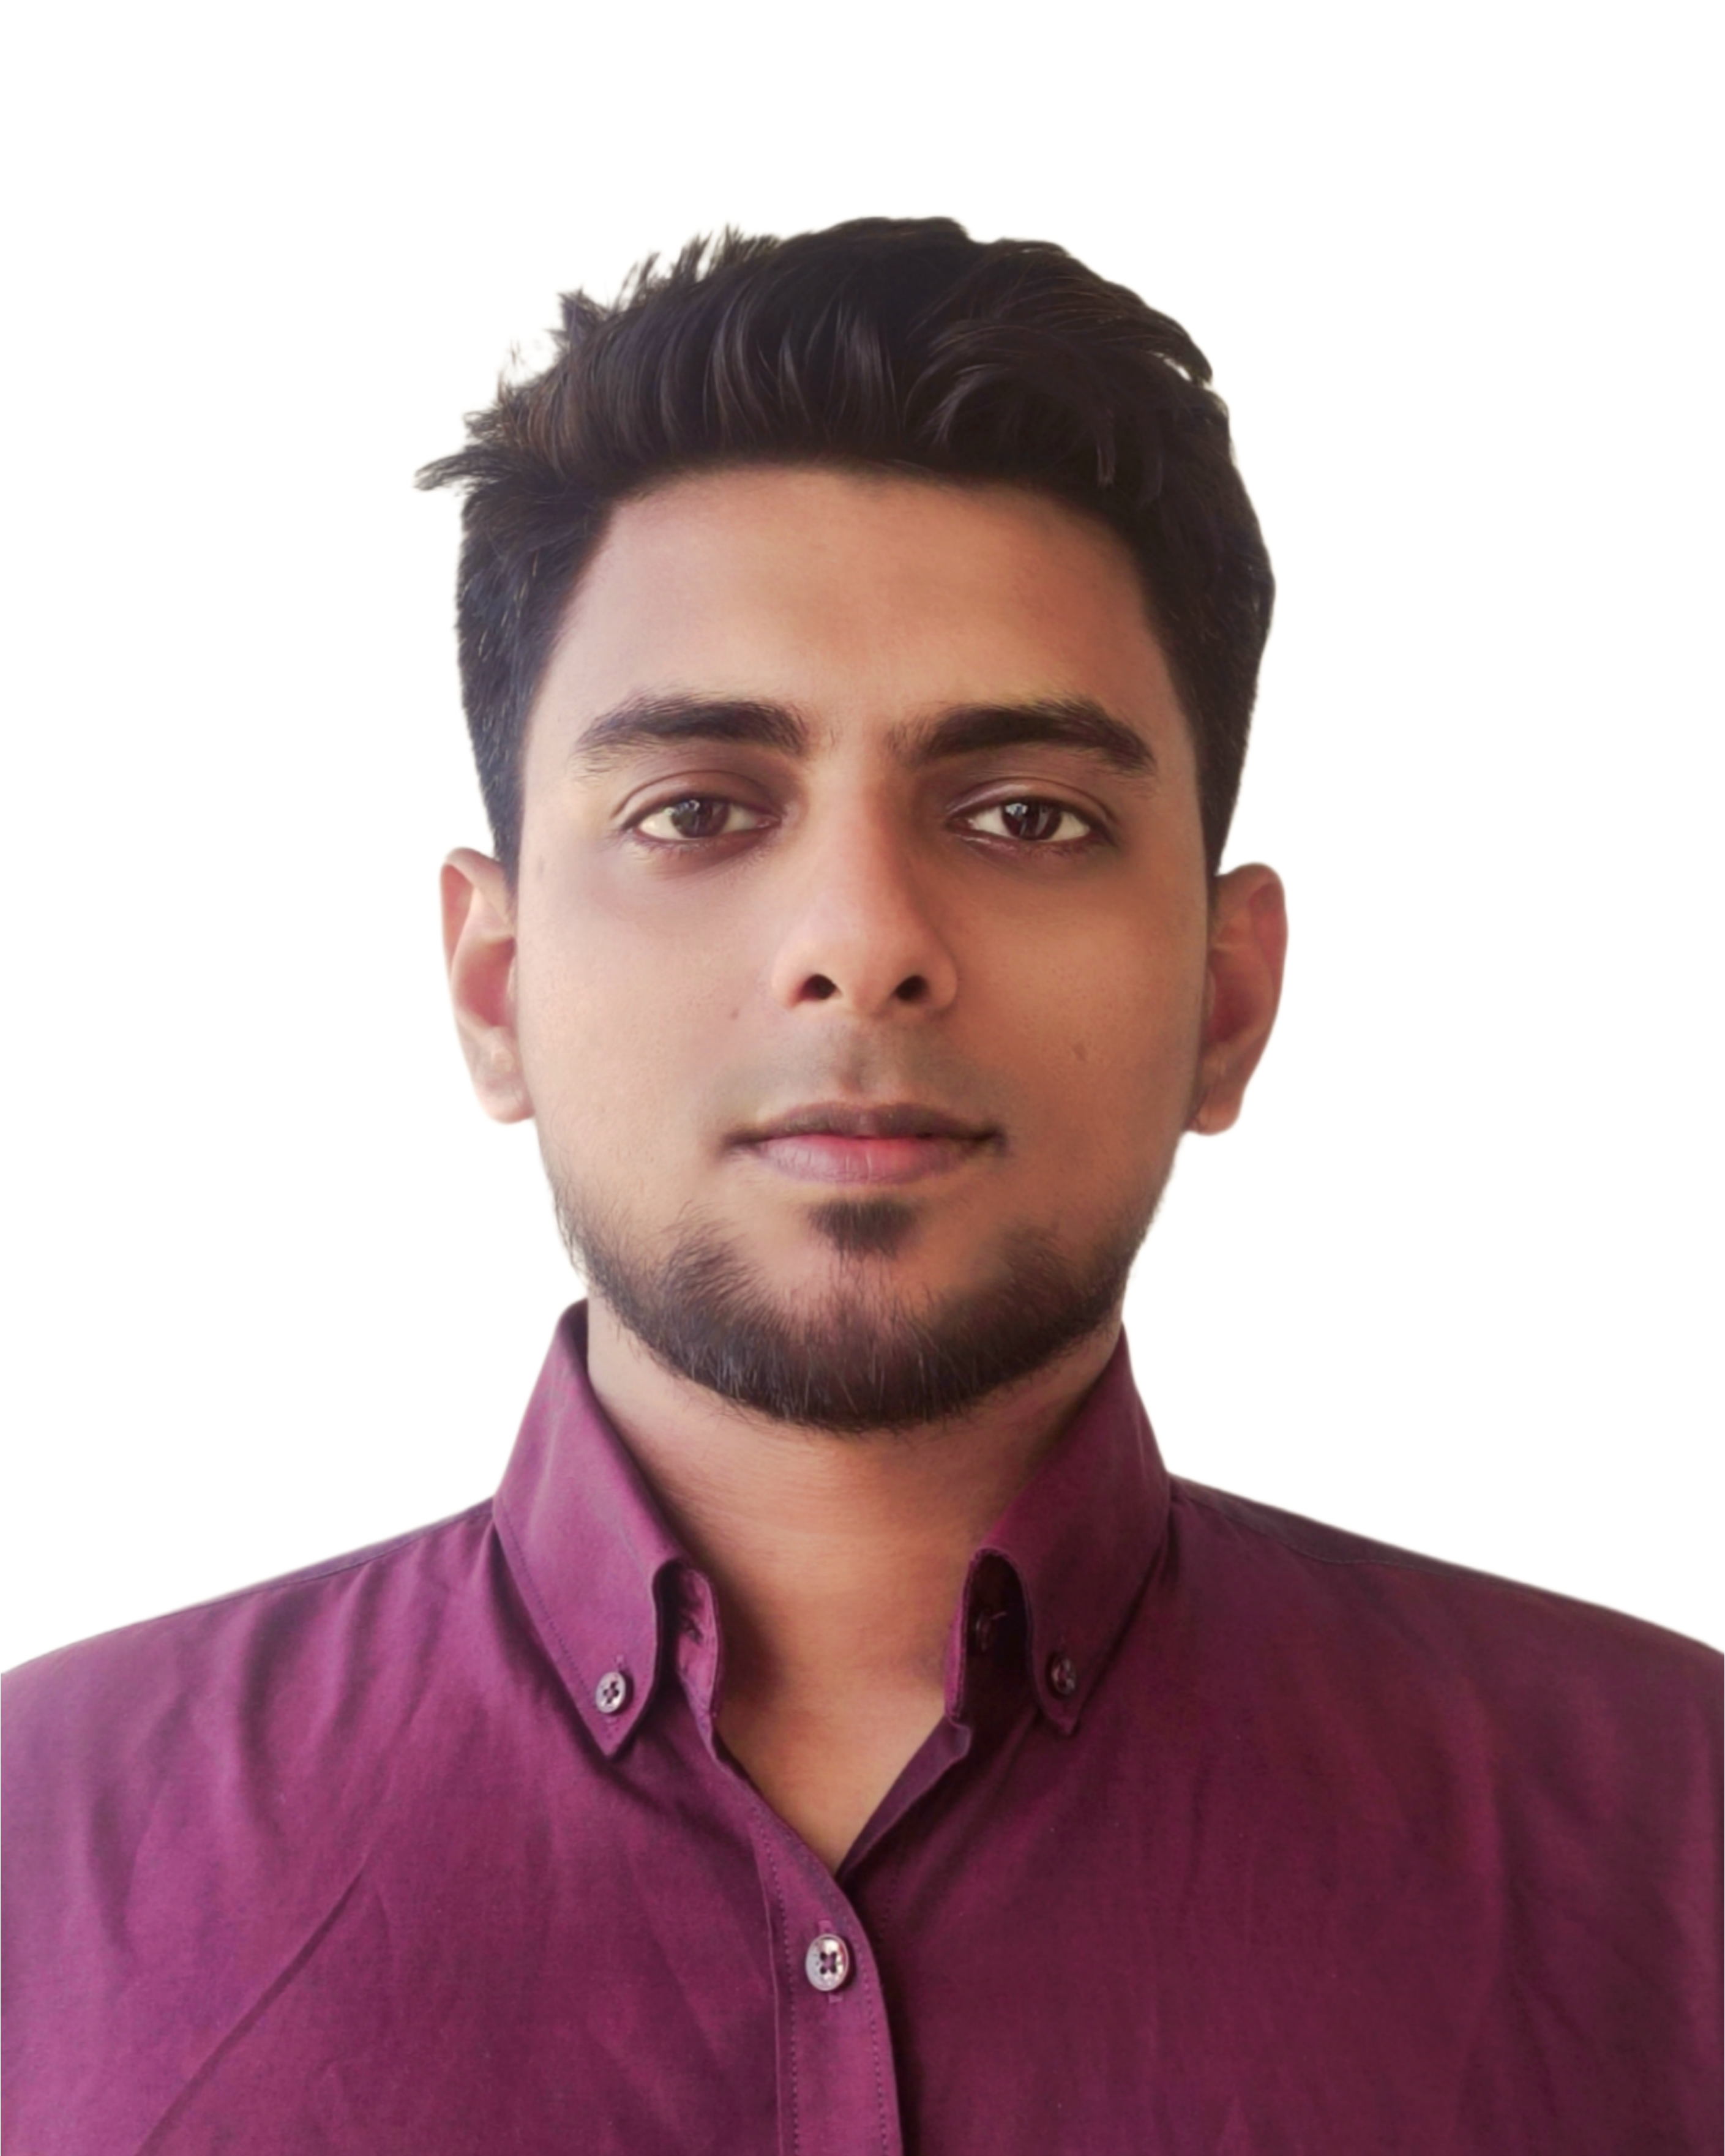
\includegraphics[width=\textwidth]{resume_image.png}
    \end{minipage}
\end{tabularx}
\vspace{-10pt}

%%%%%%%%%%%%%%%%%%%%  Career Objectives  %%%%%%%%%%%%%%%%%%%%
% \section{Career Objective}
% \justify
% To use my in-depth expertise and enthusiasm for computer science and engineering to help students through mentorship and high-quality instruction. To improve the academic programs and better equip students for fruitful careers in the sector, I hope to share my expertise in curriculum creation, research, and innovation as well as develop my technical knowledge and skills on Computer Science.

%%%%%%%%%%%%%  Professional Experiences  %%%%%%%%%%%%%
\section{Professional Experiences}
\resumeSubHeadingListStart

    %  %item-1: Fiftytwo Digital Ltd
    \resumeSubheading
    {Software Engineer}{March 2025 -- Present}
    {Fiftytwo Digital Ltd.}{Dhaka, Bangladesh}
    \vspace{-12pt}
    \ExperienceItemListStart
        \resumeItemSmall{Developing 52Vikings POS for Fitytwo A/S, Denmark} \vspace{-2pt}
        \resumeItem{\textbf{Skills: C++, SQLite}}
    \ExperienceItemListEnd

    %item-1: Brain Station 23
    \resumeSubheading
    {Software Engineer I}{March 2024 -- Present}
    {Brain Station 23 PLC.}{Dhaka, Bangladesh}
    \vspace{-12pt}
    \ExperienceItemListStart
        \resumeItemSmall{Developed various client websites} \vspace{-2pt}
        \resumeItemSmall{Developed various plugins for LMS} \vspace{-2pt}
        \resumeItem{\textbf{Skills: PHP, Python, Laravel, Django, WordPress, MySQL, PostgreSQL}}
    \ExperienceItemListEnd

    % %item-1: Brain Station 23
    % \resumeSubheading
    % {Associaite Software Engineer}{March 2024 -- Present}
    % {Brain Station 23 PLC.}{Dhaka, Bangladesh}
    % \vspace{-12pt}
    % \resumeItemListStart
    %     \resumeItemSmall{Developed various client websites} \vspace{-2pt}
    %     \resumeItemSmall{Developed various plugins for LMS} \vspace{-2pt}
    %     \resumeItem{\textbf{Skills: PHP, Laravel, Moodle, WordPress}}
    % \resumeItemListEnd

  \resumeSubHeadingListEnd

%%%%%%%%%%%%%%%%%%%%  Education  %%%%%%%%%%%%%%%%%%%%
\section{Education}
\resumeSubHeadingListStart

    % Khulna University of Engineering & Technology
    \resumeSubheading
    {Bachelor of Science in Computer Science}{CGPA -- 3.81/ 4.00}
    {Khulna University of Engineering \& Technology}{2019 -- 2024}
    \vspace{-9pt}

    % Notre Dame College, Dhaka
    \resumeSubheading
    {Higher Secondary School Certificate}{GPA -- 5.00/ 5.00}
    {Notre Dame College, Dhaka}{2016 -- 2018}
    \vspace{-9pt}

    % Monipur High School & College
    \resumeSubheading
    {Secondary School Certificate}{GPA -- 5.00/ 5.00}
    {Monipur High School \& College}{2006 -- 2016}
\resumeSubHeadingListEnd

%%%%%%%%%%%%%%%%%%  Relevent Courses  %%%%%%%%%%%%%%%%%%
% \section{Relevent Courses}
%         \begin{multicols}{3}
%             \begin{itemize}[itemsep=-2pt, parsep=3pt]
%                 \item Object Oriented Programming
%                 \item Data Structures and Algorithms
%                 \item Software Engineering
%                 \item Database Management Systems
%                 \item Computer Networks
%                 \item Operating Systems
%             \end{itemize}
%         \end{multicols}

%%%%%%%%%%%%%%%%%%%%  Thesis and Researchs  %%%%%%%%%%%%%%%%%%%%
\section{Research and Publications}
\resumeSubHeadingListStart

    % Research: 1
    \researchProjectItem
    {
        %title
        \textbf{An Analysis on Structural MRI Images for Better Alzheimer Disease Detection using Deep Neural Networks}
        % Necessary Technology
         $|$ \emph{\small Deep learning, CNN, Python, Tensorflow, OpenCV}
        % Paper Link
        $|$ \href{https://dl.acm.org/doi/10.1145/3723178.3723302}{\textcolor{urlcolor}{\small Link}}
    }
    %
    % Time of Research
    {January, 2024}
    % Description
    {The objective of the research work is to classify different stages of Alzheimer's Disease from structural MRI using CNN based model. This research work has been published in the International Conference on Computing Advancements (ICCA), 2024.}

    % % Research: 2
    % \researchProjectItem
    % {
    %     %title
    %     \textbf{An Analysis on Structural MRI Images for Better Alzheimer Disease Detection using Deep Neural Networks}
    %     % Necessary Technology
    %      $|$ \emph{\small Deep learning, CNN, Python, Tensorflow, OpenCV}
    % }
    % % Time of Research
    % {January, 2025}
    % % Description
    % {The objective of the research work is to classify different stages of Alzheimer's Disease from structural MRI using CNN based model. This research work is being reviewed by International Conference on Computing Advancements - ICCA 2024.}

\resumeSubHeadingListEnd

%%%%%%%%%%%%%%%%%%%%  Thesis and Researchs  %%%%%%%%%%%%%%%%%%%%
\section{Major Projects}
\resumeSubHeadingListStart
    % Research: 1
    \researchProjectItem
    {
        % Title
        \textbf{motoXchange}
        % Necessary Technology
        $|$ \emph{\small PHP, HTML, CSS, JavaScript, MySQL}
        % Project Link
        $|$ \href{https://github.com/RIfatArefin32/motoXchange}{\textcolor{urlcolor}{\small Project Link}}
    }
    % Time of Research
    {January, 2025}
    % Description
    {A web platform where people can buy, sell and exchange their used cars. It is developed using HTML, CSS, JavaScript and PHP without using any framework.}

    % Research: 2
    % \researchProjectItem
    % {
    %    % title
    %     \textbf{Service-Now}
    %     % Necessary Technology
    %     $|$ \emph{\small Flutter, Dart, Google Map API}
    %     % Project Link
    %     $|$ \href{https://github.com/RifatArefin32/Service-Now-Merge-User-Provider}{\textcolor{urlcolor}{\small Project Link}}
    % }
    %  % Time of Research
    % {September, 2022}
    % % Description
    % {This is a dynamic service application. In this project, there are several providers who provide services in response to service call from customers. The location of service seeker and the provider}

    %%%%%% Project: Asset Management System %%%%%%
    % \researchProjectItem
    % {
    %     % Title
    %     \textbf{Asset Management System}
    %     % Necessary Technology
    %     $|$ \emph{\small PHP, Laravel, HTML, CSS, JavaScript, MySQL}
    %     % Project Link
    %     $|$ \href{https://github.com/RifatArefin32/Asset-Management-System}{\textcolor{urlcolor}{\small Project Link}}
    % }
    % % Time of Research
    % {March, 2024}
    % % Description
    % {This project is developed based on Snipe-IT; an open-source IT asset management system. I customized Snipe-IT project according to the additional requirements.}

    \researchProjectItem
    % title
    {\textbf{Buffalo Burger}
    % Necessary Technology
    $|$ \emph{\small Java, JavaFx, MySQL}
    % Project Link
    $|$ \href{https://github.com/RifatArefin32/Buffalo-Burger}{\textcolor{urlcolor}{\small Project Link}}
    }
    % Time of Research
    {June, 2021}
    % Description
    {A desktop application using JavaFx which is basically a cloud restaurant management system that has customer interface and admin control as well.}

    % \researchProjectItem
    % % title
    % {\textbf{Mahjong Tiles}
    % % Necessary Technology
    % $|$ \emph{\small Python, Tkinter}
    % % Project Link
    % $|$ \href{https://github.com/RifatArefin32/Mahjong-Tiles_AI-Game}{\textcolor{urlcolor}{\small Project Link}}
    % }
    % % Time of Research
    % {June, 2023}
    % % Description
    % {This is a game project developed in python. This is a two players game project. User can play with computer as well. Computer moves are determined by minimax algorithm and alpha-beta pruning.}

    \researchProjectItem
    % title
    {\textbf{3D food court design}
    % Necessary Technology
    $|$ \emph{\small C, OpenGL 3.3}
    % Project Link
    $|$ \href{https://github.com/RifatArefin32/Mahjong-Tiles_AI-Game}{\textcolor{urlcolor}{\small Project Link}}
    }
    % Time of Research
    {November, 2023}
    % Description
    {Computer Graphics project in OpenGL that incorporates the basic theories of Computer Graphics. This project reflects a 3D design idea of a food court that comprises different shops selling varieties of foods and open space for customers to sit down and enjoy their times.}

    % \researchProjectItem
    % % title
    % {\textbf{Online Car Showroom Database Management System}
    % % Necessary Technology
    % $|$ \emph{\small SQL, PLSQL}
    % % Project Link
    % $|$ \href{https://github.com/RIfatArefin32/Online-Car-Showroom-Database-Management-System}{\textcolor{urlcolor}{\small Project Link}}
    % }
    % % Time of Research
    % {July, 2022}
    % % Description
    % {A database management project that includes almost all necessary queries to maintain a Car Showroom.}

\resumeSubHeadingListEnd

%%%%%%%%%%%%%%%%%%  Technical Skills  %%%%%%%%%%%%%%%%%%
\section{Technical Skills}
\resumeItemListStart
    \resumeItem{\textbf{Programming Languages: }C, C++, PHP, HTML, CSS, JavaScript, Python, Java}
    \vspace{-6pt}
    \resumeItem{\textbf{Web App Development: }Laravel, WordPress, Moodle}
    \vspace{-6pt}
    \resumeItem{\textbf{Mobile App Development: }Android Studio, Flutter}
    \vspace{-6pt}
    \resumeItem{\textbf{Other tools and frameworks: }MySQL, Git \& Github, OpenCV, Tensorflow, OpenGL}
\resumeItemListEnd

%%%%%%%%%%%%%%%%%%  Problem Solving Achievements  %%%%%%%%%%%%%%%%%%
\section{Problem Solving Achievements}
\justify
Solved \textbf{1200+} programming problems and participated onsite and online programming contests.
\vspace{-5pt}
\resumeItemListStart
    \resumeItem{\textbf{Codeforces:} \textcolor{urlcolor}{\href{https://codeforces.com/profile/3_aRrIeFfAiTn_2}{3\_aRrIeFfAiTn\_2}}, \textbf{Max Rating 1370}, Solved 800+ problems}
    \vspace{-6pt}
    \resumeItem{\textbf{AtCoder:} \textcolor{urlcolor}{\href{https://atcoder.jp/users/RifatArefin32}{RifatArefin32}}, Solved 200+ problems.}
    \vspace{-6pt}
    \resumeItem{\textbf{LeetCode:} \textcolor{urlcolor}{\href{https://leetcode.com/RifatArefin32/}{RifatArefin32}}, Solved 150+ problems.}
    \vspace{-6pt}
    \resumeItem{\textbf{LightOJ:} \textcolor{urlcolor}{\href{https://lightoj.com/user/rifat_arefin32}{rifat\_arefin32}}, Solved 50+ problems.}
\resumeItemListEnd

%%%%%%%%%%%%%%%%%%  Achievements  %%%%%%%%%%%%%%%%%%
\section{Achievements}
 \resumeItemListStart
    \resumeItem{\textbf{DEAN’s Awards, Faculty of EEE, } Session 2019-20, 2020-21 and 2021-22}
    \vspace{-6pt}

    \resumeItem{\textbf{KUET Technical Scholarships, } Session 2019-20, 2020-21 and 2021-22}
    \vspace{-6pt}

    \resumeItem{\textbf{Best Team from 2k18 Batch, position-11, } Intra KUET Programming Contest 2022}
    \vspace{-6pt}

    \resumeItem{\textbf{Board Scholarships, } Dhaka Education Board}
\resumeItemListEnd

%%%%%%%%%%%%%%%%%%  Extra Curricular Activities  %%%%%%%%%%%%%%%%%%
\section{Extra Curricular Activities}
\resumeItemListStart
    \resumeItem{\textbf{Workshop Manager, } Hardware Acceleration Club of KUET (HACK)}
    \vspace{-6pt}
    \resumeItem{\textbf{Joint Secretary, } Bit2Byte (Research \& Development Club of KUET)}
    \vspace{-6pt}
    \resumeItem{\textbf{Senior Mentor (Boys), } Special Group Interested in Programming Contest (SGIPC)}
\resumeItemListEnd

%%%%%%%%%%%%%%%%%%  Personal Information  %%%%%%%%%%%%%%%%%%
% \section{Personal Information}
% \resumeItemListStart
%     \resumeItem{\textbf{Father's Name:} Md. Ali Haider}
%     \vspace{-6pt}
%     \resumeItem{\textbf{Mother's Name:} Manija Haider}
%     \vspace{-6pt}
%     \resumeItem{\textbf{Date of Birth:} 04 March, 2000}
%     \vspace{-6pt}
%     \resumeItem{\textbf{Gender:} Male}
%     \vspace{-6pt}
%     \resumeItem{\textbf{Marital Status:} Married}
%     \vspace{-6pt}
%     \resumeItem{\textbf{Religion:} Islam}
%     \vspace{-6pt}
%     \resumeItem{\textbf{Nationality:} Bangladeshi}
%     \vspace{-6pt}
%     \resumeItem{\textbf{Permanent Address:} Vill: Anupampur, P.S. + P.O.: Charghat, Dist.: Rajshahi}
%     \vspace{-6pt}
%     \resumeItem{\textbf{Present Address:} Road-1, House-2, Block-F, Mirpur-2, Dhaka-1216}
%     \vspace{-6pt}
%     \resumeItem{\textbf{Language:} Bengali, English}
% \resumeItemListEnd

%%%%%%%%%%%%%%%%%%  References  %%%%%%%%%%%%%%%%%%
\section*{References}
\vspace{2pt}
    \setlength{\columnsep}{50pt}
    \begin{multicols}{2}

    \noindent
    %%%%%% Teacher 1 %%%%%
    % \textbf{Dr. M.M.A. Hashem} \\
    % Professor \\
    % Department of Computer Science and Engineering,\\
    % Khulna University of Engineering \& Technology (KUET) \\
    % Phone: +880 1714-003949 \\
    % Email: hashem@cse.kuet.ac.bd \\
    \textbf{Dr. Sk. Imran Hossain} \\
    Associate Professor \\
    Department of Computer Science and Engineering,\\
    Khulna University of Engineering \& Technology (KUET) \\
    Phone: +880 1758073936 \\
    Email: imran@cse.kuet.ac.bd

    \columnbreak
    \noindent
    %%%%%% Teacher 2 %%%%%
    \textbf{Dr. Al Mahmud} \\
    Associate Professor \\
    Department of Computer Science and Engineering,\\
    Khulna University of Engineering \& Technology (KUET) \\
    Phone: +880 1924332593 \\
    Email: mahmud@cse.kuet.ac.bd

    % \textbf{Abdul Aziz} \\
    % Assistant Professor \\
    % Department of Computer Science and Engineering,\\
    % Khulna University of Engineering \& Technology (KUET) \\
    % Phone: +880 1753258105 \\
    % Email: abdulaziz@cse.kuet.ac.bd

    \end{multicols}

\end{document}
%%%%%%%%%%%%%%%%%%  RESUME Ends Here  %%%%%%%%%%%%%%%%%%
